\subsection{Espectro electromagnético}

El \textbf{espectro electromagnético} es la distribución de todas las formas posibles de radiación electromagnética, ordenadas según su frecuencia o longitud de onda. Comprende desde las ondas de radio, con longitudes de onda muy largas y baja frecuencia, hasta los rayos gamma, con longitudes de onda extremadamente cortas y alta frecuencia.

Toda radiación electromagnética es una forma de energía que se propaga en el espacio en forma de ondas que combinan campos eléctricos y magnéticos perpendiculares entre sí y a la dirección de propagación. Estas ondas no requieren de un medio material para propagarse.

El espectro electromagnético se divide, en términos generales, en las siguientes regiones:

\begin{figure}[ht]
  \centering
  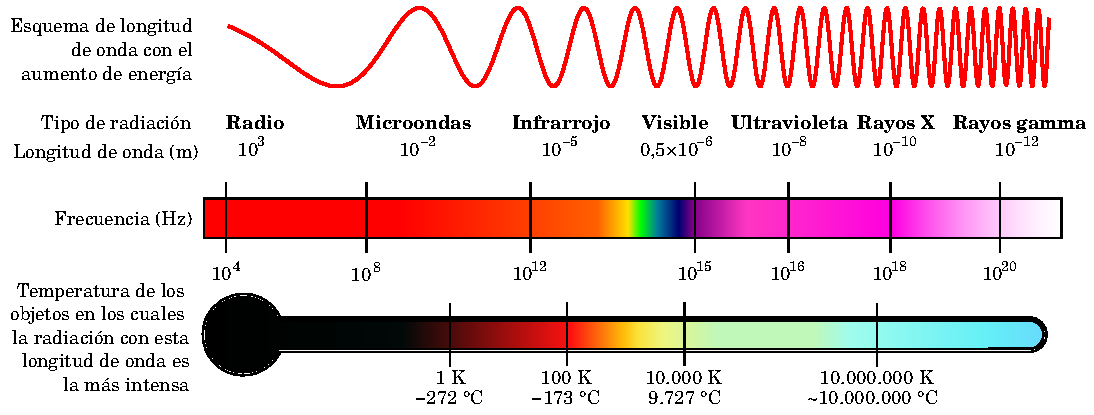
\includegraphics[width=1\textwidth]{em_spectrum.pdf}
  \caption{Espectro electromagnético}
  \label{fig:em_spectrum}
\end{figure}

Cada región del espectro tiene aplicaciones tecnológicas y científicas específicas. Por ejemplo, las ondas de radio se utilizan en telecomunicaciones, el infrarrojo en sensores térmicos, la luz visible en iluminación y visión, los rayos X en medicina, y los rayos gamma en tratamientos oncológicos.

En la figura \ref{fig:em_spectrum} se puede ver el espectro electromagnético ordenado según su longitud de onda. Vemos que a medida que la longitud de onda disminuye, la frecuencia aumenta. Esto es porque la longitud de onda y la frecuencia son inversamente proporcionales:
\[
  \lambda \propto \frac{1}{f}
\]
como vimos recién en la sección \ref{sec:maxwell_electromagnetismo} donde Maxwell demostró que la velocidad de la luz en el vacío es constante y es la misma para todas las regiones del espectro electromagnético. Por lo tanto, la longitud de onda y la frecuencia están relacionadas por la velocidad de la luz \(c\):
\[
  \lambda \cdot f = c = 299792458 \text{ m/s}
\]